\section{\eris\ simulation}

%% Introduction (ref Guedes11)
\eris\mycite{guedes11e} is a N-body/smooth particle hydrodynamics simulation of a galaxy forming in $\Lambda$CDM cosmology (see section \ref{sec:cosmology}.

%% SPH
%% - particle-sim
%% - meshgrid-sim
%% - combination (sphere of gas/kernel, hydrodynamical effects)
%% - tree structure (map distances, mass-center for far-away distances)
%% - gasoline (general, cooling, dynamical timestepping, drop layers-paragraph)
%% - \comment{add to introduction - pure DM vs. gas vs. postproduction}
%% - references to SPH-article and Gasoline-article
%% - eqs of gravity, momentum, continuity, thermal energy(, poisson?)
%% - figs sph/gasoline?

%% Details + properties eris
The simulation consist of dark matter particles and baryonic gas
particles. Star particles are created when the number density
passes 5 atoms cm$^{-3}$\footnote{Assuming three quarter neutral hydrogen and one quarter neutral helium, by mass, this threshold density equals $0.043\msol pc^{-3}$. A gas particle is initially represented by a total mass of $2\times10^{4}\msol$ and a smoothing length/radius of \importantcomment{Dafuq is the smoothing length}.}. Feedback from an active galactic nucleus
is neglected, but supernova-feeback is considered along with
cosmic UV background and radiative cooling.

Some properties of the simulated galaxy:
\begin{itemize}
\item{rotaional disk with scale length $R_d=2.5kpc$}
\item{``gentle'' rotation curve with circular velocities up to 2.2
  scale lengths}
\item{i-band (infrared wavelength 806 nm, bandwidth 149 nm)
  bulge-to-disk-ratio of $B/D=0.35$}
\item{baryonic mass fraction inside halo is 30\% lower then
  cosmic average}
\item{thin disk with typical HI-stellar mass-ratio}
\item{disk is forming stars in $\Sigma_{sfr}-\Sigma_{HI}$ plane}
\item{disk falls on photometric Tully-Fisher relation and
  stellar mass - halo virial mass relation}
\item{structural properties, mass budget, and scaling relations between mass and luminosity matches several observational constraints}
\end{itemize}

%% ``Angular momentum problem'' description + solution + sources
\subsection{Angular momentum problem}
In galactic simulations there is an ``angular momentum problem''. This refers to baryonic components having much less rotaional spin in simulations than real observations. This failure was believed to arise from friction moving angular momentum from sub-structures to outer halo when these sub-structures merge causing the cold clumps of gas to fall to the center\mycite{navarro91}.
Meaning that cosmological simulation with gas become clumped in the center of halos, instead of forming disks like observed galaxies. The ``problem'' being not enough angular momentum in the gas.
In newer times this problem have been attempted solved with energy injected from supernovae, meaning evolving stars from the gas content to decrease the effect of cooling and removing angular moment from the center of the galaxy. The stars heat the surrounding gas, and the supernovae add kinetic energy to the gas so it is not allowed to cluster too much in the center.

%% Fig galaxy-sheet

\begin{figure}
  \centering
  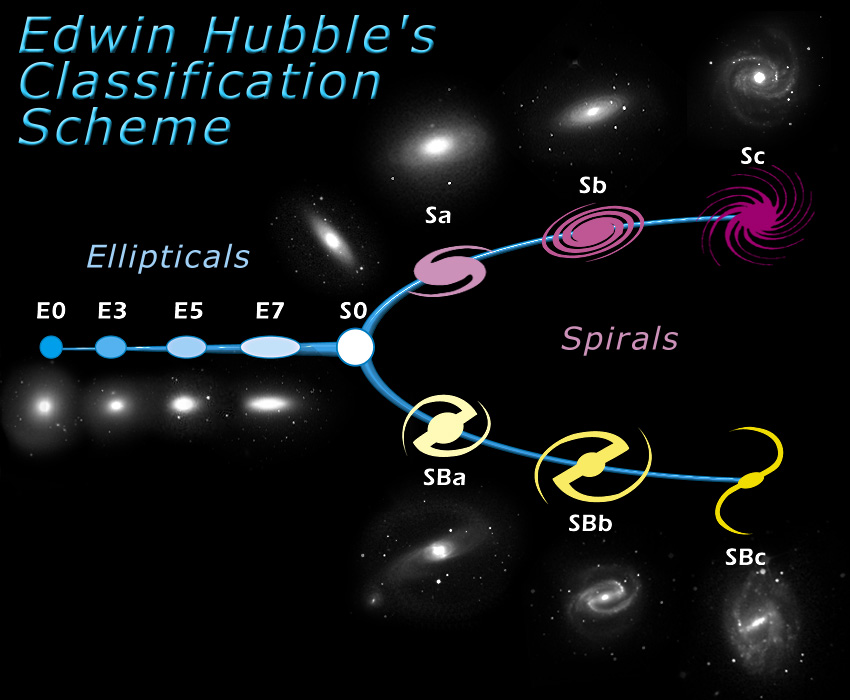
\includegraphics[width=\figwidth]{img/HubbleTuningFork.jpg}
  \caption{\ref{img:HubbleTuningFork}
    The Hubble morphological classification of galaxies from their observed shape. Described either as elliptical, spherical or spherical with a bar in the center.
    Source: ESA
  }
\end{figure}


%% What eris present (figs?)
\mycite{guedes11e} presents a realistic simulation of a Milky Way type galaxy using a new smooth particle hydrodynamic cosmological simulation called \eris, based on \gasoline\mycite{wadsley03}. It includes radiative cooling, cosmic UV heating, supernova feedback, and high-density star formation requirement (which is believed to be a key ingredient in producing realistic spirals in galactic simulations).
The high density threshold for star formation (5 atoms cm$^{-3}$) creates sparsely, clustered regions of star formation that remove low-angular momentum cold gas from the center of the halo. 
%% postprocessing (ref Shen15)
%% - implementaion
%% - conclusion (add GW170817 observation)
%% - figs Eu-t, Eu-z
%% - figs SFR, NSMR

By using the \eris-simulation, the chemical evolution of the milky way is studied.
\eris\ traces oxygen and iron from supernovae.
\mycite{shen15} postprocesses the simulation data from \eris\ to include neutron star mergers that add europium (an r-process tracer) to the interstellar medium.
The study shows that the heavy products of neutron star mergers can be incorporated into early stars, even if the shortest neutron star mergers is 100 Myr. The conclusion of the study does not vary much with delay-time and merger rate and an argument is made for neutron star mergers being the dominant r-process source in the galaxy.

This is supported by the neutron star merger (GW170817) observed\mycite{GW170817}. With \textit{estimated} dynamical ejecta of mass 0.002\msol and velocity of 0.2c and highspeed wind ejecta of mass 0.015\msol and velocity of 0.08c. Such velocities are high enough to cross a galaxy within $\simeq 1$ Gyr, and if most of the ejecta manifests as r-process material the assumed model of \mycite{shen15} (ejected r-process material of 0.01\msol) is realistic. The single GW170817 observation makes rate of such events hard to estimate, and therefore difficult to constrain the neutron star merger rate in \eris.

%% Move stuff to theory I section
Looking at very metal poor stars in our Galaxy, which have been around for a long time. r-process abundances can be found. Meaning that the source of r-process has been around for a long time, and in a robust manner. However, the large variations show that the process was unhomogenous for early times, while it is moore smoothed after many Galactic rotations and repeated events.
The two main regions of producing these heavy r-process elements are in the merger of two neutron stars (or the merger between a neutron star and a black hole) or in a heavy core collapse supernova. The production yields are much larger for neutron star mergers, but they are also much more rare.
(Important citations Takashi94 and Woosley94 for SNII; Lattimer 77 and Freiburghaus 99 for NSM)

%% chemical observations
The neutron star merger events are set to occur near the stellar distribution, and since the kinetic energy outout is not large compared to supernovae the gas dynamics is unaffected.
In simple terms, the neutron star mergers are injected in stellar regions and therefor drown in the bright, explosive environment of larger supernovae.

Using the time evolution of the star formation rate, the neutron star merger events are injected at random star-particles (simple stellar populations).

At redshift zero the oxygen-iron abundances can be split into two main regions. One primarily enriched by type II supernovae, which are more rich in oxygen, leading to higher (supersolar) ratios. Another which are primarily enriched by type Ia supernovae, leading to more iron than oxygen.

There are two main implementations involved, one without any mixing, and another with mixing of metals between gas particles. For both oxygen-iron ratios and europium-iron ratios one sees that mixing gives less variation between ``upper'' and ``lower'' sigma-bands.

Populating some star particles with neutron star mergers and have them enrich the nearby gas particles, and subsequentually the new star particles, gives a more complete abundance-pattern to trace.
The abundances traced are hydrogen, oxygen (which primarily follows type II supernovae), iron (produced more abundently in type Ia supernovae) and europium (produced in neutron star mergers only). The europium-iron ratio varies widely, even for early times.

r-process nucleosynthesis requires neutron heavy isotopes, and the two leading theories are neutron star mergers and type II supernovae (see references Burbridge 1957, Roberts 2010, Lattimer 1977). Even though the conditions of the neutron star environment are somewhat uncertain, estimates are promising for the neutron star mergers to produce heavy isotopes in r-process distributions.
These two processes, neutron star mergers and type II supernovae are quite different in frequency and yields, meaning that galactic chemical evolution models should be able to predict which of the models are most likely.

The chemical enrichment is closely tied to the star formation rate/history/birth/death, and thereby makes the 'Eris' simulation a good approximation for the Milky Way Galaxy.
This study (shen15 'Eris' rncp post-production) finds that neutron star mergers are capable of enriching the surrounding medium, even with a minimum delay-time of 100 Myr.

The dispersion/variantion of [Eu/Fe] is great enough, even at low metallicities.
The results changing the parameters in the fiducial model is obvious, and I've elaborated on this before.
The conclusion is that variations of the model parameters do not significantly alter the result.
The mixing level affects the abundance of europium, but it is hard to compare to observations becasue spectroscopic abundance of many stars are unknown.

Galactic chemical evolution models are single points in space with mass resolution and time-integration. These models are simple way of calculating the mean amount of elements in the galaxy based on a star formation history, yield tables and initial composition.
These models do not replicate the inhomogeneities and variations in metal-distributions.
An attempt is made in this study to reproduce the results with a 1D-model based on the parameters used in Eris.
At late times model agrees well with the average of all of Eris, however it does not agree well with the early results of Eris, nor does it replicate the large variations in spectroscopic abundance during early times.

\iffalse
\importantcomment{This section is outdated as of 10.05.18}

\section{\eris simulation}

'Eris' is a N-body/smooth particle hydrodynamics simulation of a
galaxy forming in $\Lambda$CDM cosmology.
The simulation consist of dark matter particles and baryonic gas
particles. Star particles are created when the number density
passes 5 atoms cm$^-3$. Feedback from an active galactic nucleus
is neglected, but supernova-feeback is considered along with
cosmic UV background and radiative cooling.

Some properties of the simulated galaxy:
\begin{itemize}
\item{rotaional disk with scale length $R_d=2.5kpc$}
\item{``gentle'' rotation curve with circular velocities at 2.2
  scale lengths}
\item{i-band (infrared wavelength 806 nm, bandwidth 149 nm)
  bulge-to-disk-ratio of $B/D=0.35$}
\item{baryonic mass fraction inside halo is 30\% lower then
  cosmic average}
\item{thin disk with typical HI-stellar mass-ratio}
\item{disk is forming stars in $\Sigma_{sfr}-\Sigma_{HI}$ plane}
\item{disk falls on photometric Tully-Fisher relation and
  stellar mass - halo virial mass relation}
\item{structural properties, mass budget, and scaling relations between mass and luminosity matches several observational constraints}
\end{itemize}

In galactic simulations there is an ``angular momentum problem''. This refers to baryonic components having much less rotaional spin in simulations than real observations. This failure was believed to arise from friction moving angular momentum from sub-structures to outer halo when these sub-structures merge causing the cold clumps of gas to fall to the center.
In newer times this problem have been attempted solved with energy injected from supernovae, meaning evolving stars from the gas content to decrease the effect of cooling and removing angular moment from the center of the galaxy.
Star formation in the disk comes from inflow of cold baryonic gas that was never shock heated to virial temperature.
\comment{INSERT S0...-GALAXY-SHEET.}
%link thesis/img/HubbleTuningFork.jpg

Yet the simulated galaxies have more centered baryon components and reproduce only S0 and Sa type galaxies. With two major exceptions there are no simulations of type Sb and Sc, one exception with low star formation and another with low mass.

This paper presents a realistic simulation of a Milky Way type galaxy using a new smotth particle hydrodynamic cosmological simulation. It includes radiative cooling, cosmic UV heating, supernova feedback, and high-density star formation requirement(which is believed to be a key ingridient.

The high threshold for star formation is important to create non-centered galaxies

%r-process post-production with Shen 2015
In Shen 15 \comment{(insert proper citation)} the simulation data from 'Eris' is post-processed to include, not only oxygen adn iron, but also europium from neutron star mergers.

By using the 'Eris' simulation\cite{guedes11e}, the chemical evolution of the milky way is studied.
'Eris' traces oxygen and iron from supernovae and in this work, postproduction traces neutron star mergers and the europium ejected from them post-merger.
r-process abundance is traced in the milky way proxy by the [Eu/Fe]-ratio.
The study shows that the heavy products of neutron star mergers can be incorporated into early stars, even if the shortest neutron star mergers is 100 Myr.

The conclusion of the study does not vary much with delay-time and merger rate and an argument is made for neutron star mergers being the dominant r-process source in the galaxy.

%\section{introduction}
Looking at very metal poor stars in our Galaxy, which have been around for a long time. r-process abundances can be found. Meaning that the source of r-process has been around for a long time, and in a robust manner. However, the large variations show that the process was unhomogenous for early times, while it is moore smoothed after many Galactic rotations and repeated events.
The two main regions of producing these heavy r-process elements are in the merger of two neutron stars (or the merger between a neutron star and a black hole) or in a heavy core collapse supernova. The production yields are much larger for neutron star mergers, but they are also much more rare.
(Important citations Takashi94 and Woosley94 for SNII; Lattimer 77 and Freiburghaus 99 for NSM)

%\section{methods}
%\subsection{the Eris simulation}
%Hæ?!
%\subsection{R-process production sites and injection history}
The neutron star mergers are described by delay-time distribution, merger rate, yield of r-process elements, the spatial distribution of events.
The delay-time distribution is modelled by a power-law, $P(t) \propto t^{-n}$, from some minimum timescale to the hubble-time(end of simulation).
Each neutron star merger is assumed to created some mass of r-process material, only a fraction of this material will be europium(which is used as the tracer).
The ratio of europium to r-process material is assumed to be solar(Sneden 2008), while the merger rate is calculated from scaling the star formation integral until europium-oxygen ratio equals solar ratio.

The neutron star merger events are set to occur near the stellar distribution, and since the kinetic energy outout is not large compared to supernovae the gas dynamics is unaffected.
In simple terms, the neutron star mergers are injected in stellar regions and therefor drown in the bright, explosive environment of larger supernovae.

Using the time evolution of the star formation rate, the neutron star merger events are injected at random star-particles (simple stellar populations).

%\section{r-process enrichment in the milky way}
At redshift zero the oxygen-iron abundances can be split into two main regions. One primarily enriched by type II supernovae, which are more rich in oxygen, leading to higher (supersolar) ratios. Another which are primarily enriched by type Ia supernovae, leading to more iron than oxygen.

There are two main implementations involved, one without any mixing, and another with mixing of metals between gas particles. For both oxygen-iron ratios and europium-iron ratios one sees that mixing gives less variation between ``upper'' and ``lower'' sigma-bands.

Populating some star particles with neutron star mergers and have them enrich the nearby gas particles, and subsequentually the new star particles, gives a more complete abundance-pattern to trace.
The abundances traced are hydrogen, oxygen (which primarily follows type II supernovae), iron (produced more abundently in type Ia supernovae) and europium (produced in neutron star mergers only). The europium-iron ratio varies widely, even for early times.

%\section{discussion}
r-process nucleosynthesis requires neutron heavy isotopes, and the two leading theories are neutron star mergers and type II supernovae (see references Burbridge 1957, Roberts 2010, Lattimer 1977). Even though the conditions of the neutron star environment are somewhat uncertain, estimates are promising for the neutron star mergers to produce heavy isotopes in r-process distributions.
These two processes, neutron star mergers and type II supernovae are quite different in frequency and yields, meaning that galactic chemical evolution models should be able to predict which of the models are most likely.

The chemical enrichment is closely tied to the star formation rate/history/birth/death, and thereby makes the 'Eris' simulation a good approximation for the Milky Way Galaxy.
This study (shen15 'Eris' rncp post-production) finds that neutron star mergers are capable of enriching the surrounding medium, even with a minimum delay-time of 100 Myr.

%\subsection{dependence on model parameters}
The dispersion/variantion of [Eu/Fe] is great enough, even at low metallicities.
The results changing the parameters in the fiducial model is obvious, and I've elaborated on this before.
The conclusion is that variations of the model parameters do not significantly alter the result.
The mixing level affects the abundance of europium, but it is hard to compare to observations becasue spectroscopic abundance of many stars are unknown.

%\subsection{comparison with 1d models}
Galactic chemical evolution models are single points in space with mass resolution and time-integration. These models are simple way of calculating the mean amount of elements in the galaxy based on a star formation history, yield tables and initial composition.
These models do not replicate the inhomogeneities and variations in metal-distributions.
An attempt is made in this study to reproduce the results with a 1D-model based on the parameters used in Eris.
At late times model agrees well with the average of all of Eris, however it does not agree well with the early results of Eris, nor does it replicate the large variations in spectroscopic abundance during early times.

\fi
